\documentclass{article}
\begin{document}
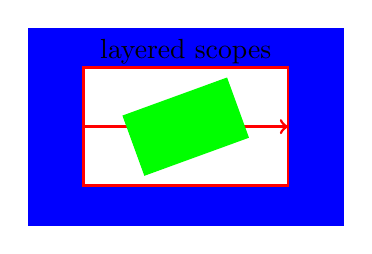
\begin{tikzpicture}
\begin{scope}[fill=blue,draw=blue]
  \filldraw (0,0) rectangle (4,2.5);
\end{scope}
\begin{scope}[fill=white]
  \fill (0.7,0.5) rectangle (3.3,2);
\end{scope}
\begin{scope}[draw=red,line width=1pt]
  \draw (0.7,0.5) rectangle (3.3,2);
  \draw[->] (0.7,1.25) -- (3.3,1.25);
\end{scope}
\begin{scope}[shift={(2,1.25)},rotate=20,draw=green,fill=green]
  \filldraw (-0.7,-0.4) rectangle (0.7,0.4);
\end{scope}
\node at (2,2.2) {layered scopes};
\end{tikzpicture}
\end{document}
